% Outlook section

\section{Outlook}

The analysis presented here is at a mature stage, but certainly not in its final for publication.  In this section, we will outline anticipated future improvements we plan to make and complementary analyses that will directly impact this result.

\subsection{Future Improvements}
\subsubsection{Track/Shower Classification}

The preceding sections showed there is significant disagreement in the track-like/shower-like classification of objects when comparing data to Monte Carlo.  In particular, the number of showers in data is higher than the number of showers in Monte Carlo, as shown in Section~\ref{sec:reclass}.  A mask is presented there to improve data/Monte Carlo agreement, by reclassifying (1) small shower-like objects as tracks based on their angular separation from the leading shower, and (2) track-like objects as showers if they are within the cone of the leading shower.  

The mask, unfortunately, is not a real solution.  Because of the difference in energy reconstruction between tracks and showers (range-based for tracks, calorimetric for showers), it's critical to the neutrino energy reconstruction to correctly identify the particles in an interaction.  Currently, we have simply ensured that the level of mis-identification between data and Monte Carlo is matched.

In principle, the track/shower misidentification issue is a collaboration-wide problem to be addressed for MCC9.  To this end, we anticipate trying short-term techniques such as BDT/SVM classifiers for TPC objects to improve classification in MCC8. Pandora itself uses an SVM classifier for track/shower separation, with good performance on Monte Carlo. By examining this training and including a data driven training set, we could improve performance on data as well. More ambitious updates from Pandora for MCC9, with the inclusion of improved signal processing and 2D deconvolution, fall under the realm of Pandora development.  We look forward to contributing to those discussions by validating and iterating on the improvements with the Pandora team.

\subsubsection{Neutrino Vertexing and Shower Splitting}

Another issue uncovered in the reconstruction of $\nu_{e}$ events is the splitting of electromagnetic showers and misplacement of the vertexes. 
Figure~\ref{fig:evd_2showers} shows an example of this problem.  

\begin{figure}[htbp]
\centering
  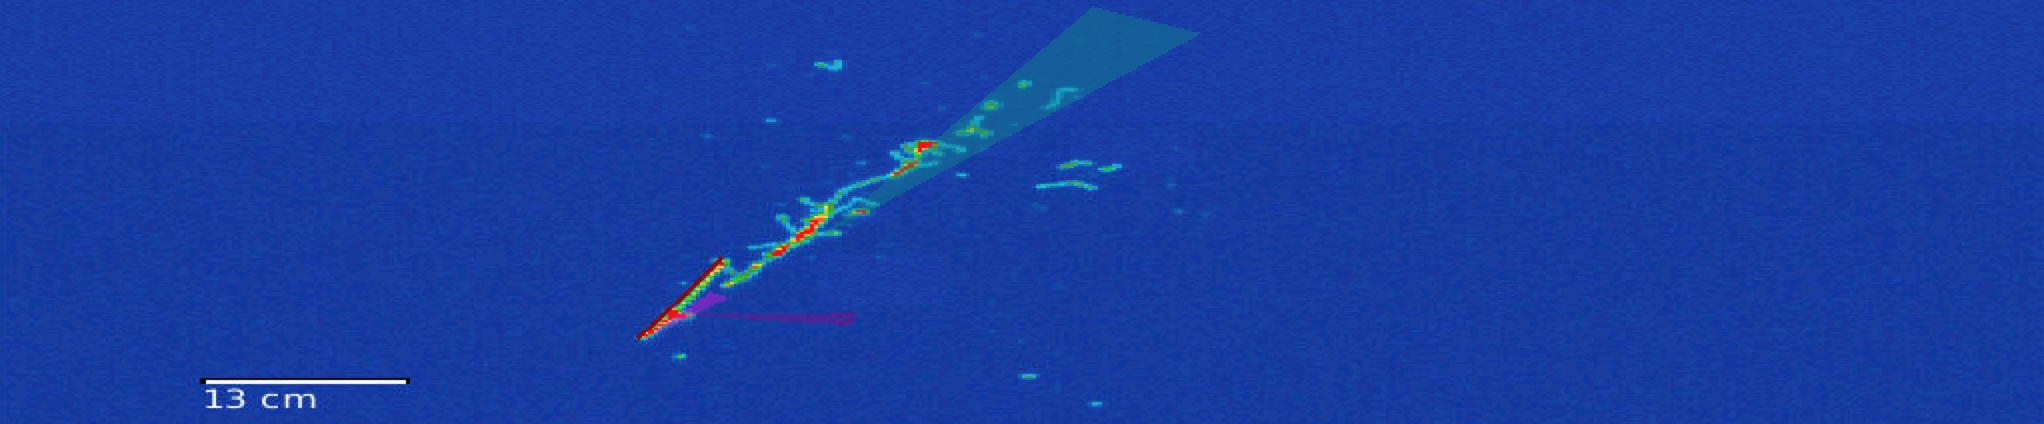
\includegraphics[width=0.7\linewidth]{figures/splitshower.png}
  \caption{Simulated event displays of the collection plane of a $\nu_{e}$ CC0$\pi$-Np event with the electron shower being split into several shower-like objects.}
  \label{fig:evd_2showers}
\end{figure}

For the low-energy excess analyses, this presents a problem for two reasons.  First, it introduces non-$\nu_{e}$ CC0$\pi$-Np events into the selected sample, since the track-like segment of an electromagnetic shower is reconstructed like a proton. Second, the splitting of a shower into multiple shower objects leads to a decreased ability to reject multi-shower events like $\pi^0\rightarrow2\gamma$ decays.

Improved clustering - particularly shower clustering - allows us to apply shower multiplicity cuts to reject background events with less aggressive cuts on the electron-like signal.

\subsubsection{Cosmic tagging with the Cosmic-ray Tagger}

In the final event distributions in Section~\ref{sec:electron_like}, the cosmic background is a sub-dominant background, due to the ability to reject these events with kinematic cuts.  However, as seen in Section~\ref{sec:numu}, the dominant source of events passing the pre-selection is cosmic-ray interactions.  The Cosmic-ray Tagger (CRT) offers several ways to reject these events at the pre-selection stage.  First, a coincidence veto of in-time flashes in the PMTs and CRT would allow us to reject a significant background of in-time cosmic events.  There is some danger that neutrino interactions are also vetoed by this coincidence, but that is unlikely for $\nu_{e}$ events - most particles that exit the TPC and can hit the CRT are muons.

Additionally, for events where an out-of-TPC neutrino interaction creates a flash in time with the beam, but a cosmic interaction is matched to that flash, the CRT can also be useful.  TPC-to-CRT matching of muon tracks can mitigate this background by flagging a TPC Pandora neutrino candidate object, and allowing us to reject out-of-time cosmic rays matched to an in-time, out-of-TPC neutrino flash.

\subsection{Complementary Analyses}

While many MicroBooNE analyses benefit this low-energy excess analysis, several in particular are directly complementary to this analysis and the coherence of their development is important to the future progress of this analysis.

\subsubsection{\texorpdfstring{$\nu_{\mu}$}{numu} Inclusive Selection}

All MicroBooNE low-energy excess searches benefit greatly from the constraint of flux, cross sections, and perhaps detector systematics by performing a joint measurement of $\nu_\mu$ and $\nu_e$ selections. In particular, the inclusive CC $\nu_\mu$ cross-section measurement described in \cite{ubxsec} also allows us to remove some $\nu_\mu$ mis-reconstructed as $\nu_e$ CC0$\pi$-Np candidates.

\subsubsection{Single Electron Inclusive Search}

Since final state interactions of neutrino's on liquid argon are not yet completely understood, a complementary $\nu_e$ CC inclusive search is ongoing. The inclusive channel is expected to be less sensitive to uncertainties in the neutrino interaction models. By not requiring the presence of a proton, theoretically, higher sensitivities at low energy are possible. Meanwhile, reconstruction and identification problems concerning protons are less important. Both the $\nu_e$ CC0$\pi$-Np and $\nu_e$ CC inclusive will share the same cosmic rejection and optical selection. The inclusive search employs particle identification using the boosted decision classifier method for electrons and muons. Reconstructed objects are tagged as electron neutrino's based on classifier using the particle identification as its input. The BNB $\nu_e$ CC inclusive search will also be compared with the ongoing NuMI $\nu_e$ CC inclusive measurement.

\subsection{Background Rejection Improvements}
The cuts described in Section \ref{sec:bkg} have two main goals: (1) ensure that the selected events are well-reconstructed, and (2) reject the background events. However, the values of each cut, even if meaningful and justified, are not optimized to the significance of the $\nu_e$ CC0$\pi$-Np component in the sample. Doing that would have left us with too few data events, making the validation of the energy spectrum shown in Section \ref{sec:electron_like} impossible. 
